% !TEX root = ../thesis.tex
\section{Porovnání člověk vs. stroj}
\label{chap:experiments:normalization}

Z experimentů provedených v části \ref{chap:experiments:analysis} vyplynula potřeba rozšířit řečový korpus. V části \ref{chap:experiments:analysis:reduction} se ukázalo, že v určitých případech jsou neznělé fonémy produkovány jako znělé. Pro lepší porozumnění tohoto jevu je nezbytné, aby řecový korpus obsahoval co možná nejvíce promluv zahrnující slova s odlišným významem, ale lišící se pouze ve znělosti právě jedonho fonému.

Tato část se zaměřuje na získání takovýchto slov a experimentů s nimi. Hlavním experimentem je porovnání schopností člověka a stroje tato slova od sebe odlišit. Na základě poznatků z tohoto experimentu jsou navrženy úpravy, které mají sloužit k zlepšení systémů rozpoznávání řeči.

Nejprve je v částu \ref{chap:experiments:normalization:corpus} popsán proces výběru a získání inkriminovaných slov a následně jsou tato nová data analyzována. V následující části \ref{chap:experiments:normalization:quality} jsou provedeny kontrolní experimenty, při kterých je zjištěn problém s přenosovým kanálem a na základě těchto zjištění je navrženo řešení. Zbylé dvě části (\ref{chap:experiments:normalization:listening} a \ref{chap:experiments:normalization:comparison}) se pak zabývají porovnáním výsledků člověka a stroje na nových datech.

\subsection{Rozšíření řečového korpusu}
\label{chap:experiments:normalization:corpus}

Před samotným nahráváním je nezbytné vybrat co možná nejvíce dvojic slov, které se liší významem a znělostí právě jednoho fonému. Příkladem může být dvojice slov \textit{kosa} + \textit{koza} nebo \textit{přibít} + \textit{přibít}. Pro tento účel je použit algoritmus výběru slov, který je následující:

\begin{enumerate}
  \item načtení dat (slovník, párové fonémy)
  \item shluknutí všech slov vedoucích ke stejné transkripci
  \item vytvoření všech možných kombinací dvojic slovních transkripcí
  \item nalezení dvojic transkripcí, které se liší právě ve znělosti jednoho fonému\footnote{Konkrétně algoritmus vzájemně porovná obě slova a najde rozdílné fonémy. Pokud tyto rozdíly odpovídají některé z dvojic párových fonémů, tak je dvojice přijata.}
  \item výběr dvojic slov na základě vybraných transkripcí
\end{enumerate}

Vstupem algoritmu je \uv{slovník} obsahující slova a jejich fonetický přepis, dále pak dvojice fonémů (znělý + neznělý). Jako slovník posloužil, v tomto konktérním případě, seznam slov s fonetickými přepisy pocházející z jazykového modelu obsahující 1,2 milionu slov. Pomocí výše zmíněného algoritmu se podařilo nalézt $160$ párů slov lišících se znělostí právě jednoho fonému, celkem tedy $320$ slov. Ke každému nalezenému slovu je následně vybrána minimálně jedna věta obsahující toto slovo (ale nikoli druhé slovo z dvojice), těchto vět je pak $418$. Příklad takto vybraných vět je uveden níže:

\begin{verbatim}
  Zkoušel jsem to několikrát, ale pokaždé padla kosa na kámen.
  Do basy nemusí, vlk žere, koza žije.
\end{verbatim}

Vybraná slova a věty jsou základem pro 2. etapu nahrávání, která se uskutečnila během dvou sezení v červenci roku 2016. Jedná se tedy o relativně velký časový odstup od 1. etapy. Nahrávání se zhostil stejný řečník jako v případě té první (viz část \ref{chap:experiments:analysis:corpus}). Samotné nahrávání bylo rozděleno do dvou samostatných sezení, mající mezi sebou týdenní rozestup. Oproti 1. etapě probíhalo nahrávání v odhlučněné nahrávácí komoře za pomocí profesionálního nahrávacího zařízení. Mikrofon byl od úst řečníka vzdálen přibližně 15 cm, protože byl použit studiový mikrofon, který kvůli své velikosti, už z podstaty, není možné přiložit přímo na tvář jako v případě 1. série nahrávání. K nahrávání byl použit speciální software, který kontroloval zda každá nahrávka splňuje určité parametry. Každá nahrávka musí mít na svém začátku a konci minimálně $0,5\ s$ ticha a zároveň celá nahrávka nesmí být příliš tichá a zároveň přebuzená (kontrolováno pomocí energie). Pokud nahrávka nesplňuje definované parametry, je zamítnuta a řečník musí promluvu zopakovat.

V části \ref{chap:experiments:analysis:corpus} je zmíněno, že je nezbytné provádět anotaci nahrávek, aby mohl být korpus kompletní. Samotná anotace je  relativně zdlouhavý proces, a proto je dobré pořídit přesné promluvy vybraných slov a vět již v průběhu nahrávání. K tomu slouží další z funkcí nahrávacího softwaru, který řečníkovi vždy ukáže text, který je potřeba vyslovit. Společně s audio záznamem je pak uložen i tento text. K dispozici je tedy nahrávka a její \uv{přepis}. Nicméně samotný řečník často může udělat chybu aniž by si toho všiml (např. záměna podobných slov apod.) a software nijak nekontroluje co je ve skutečnosti vysloveno. Z tohoto důvodu je nahrávání přítomen operátor, který poslouchá co bylo řečeno a v případě potřeby zamítné nahrávku. Řečník následně musí promluvu opakovat, dokud nahrávka neodpovídá požadovaným parametrům a zároveň je její obsah správný.

Na obr. \ref{fig:experiments:normalization:word} a \ref{fig:experiments:normalization:sentence} jsou ukázky audio záznamu slova \uv{kosa} a věty \uv{Zkoušel jsem to několikrát, ale pokaždé padla kosa na kámen.}. Pokud se nahrávky porovnají s daty získanými v 1. etapě (obr. \ref{fig:experiments:analysis:el_speech}), tak hlavním rozdílem je vyšší kvalita nahrávek, zejména vyšší amplituda. Ze zobrazených spektrogramů je zřejmé, že šum je přítomen v podobném spektru a intenzitě jako u předchozích nahrávek. Rozdíl je zejména v nižších frekvencích řeči, které jsou na spektrogramu výraznější. Přestože se jedná o stejného řečníka, tak zaznamenaná řeč nemá úplně identické parametry. Hlavním důvodem bude nepochybně změna nahrávací aparatury a procesu nahrávání. Nezanedbatelný vliv bude mít i relativní nestálost prametrů EL řeči, zvlášť v delším časovém období. Kvalita a parametry EL řeči jsou totiž velmi závislé na typu a pozici elektrolarynxu, ten se v době mezi nahráváními navíc změnil.

\begin{figure}[hbpt]
  \centering
  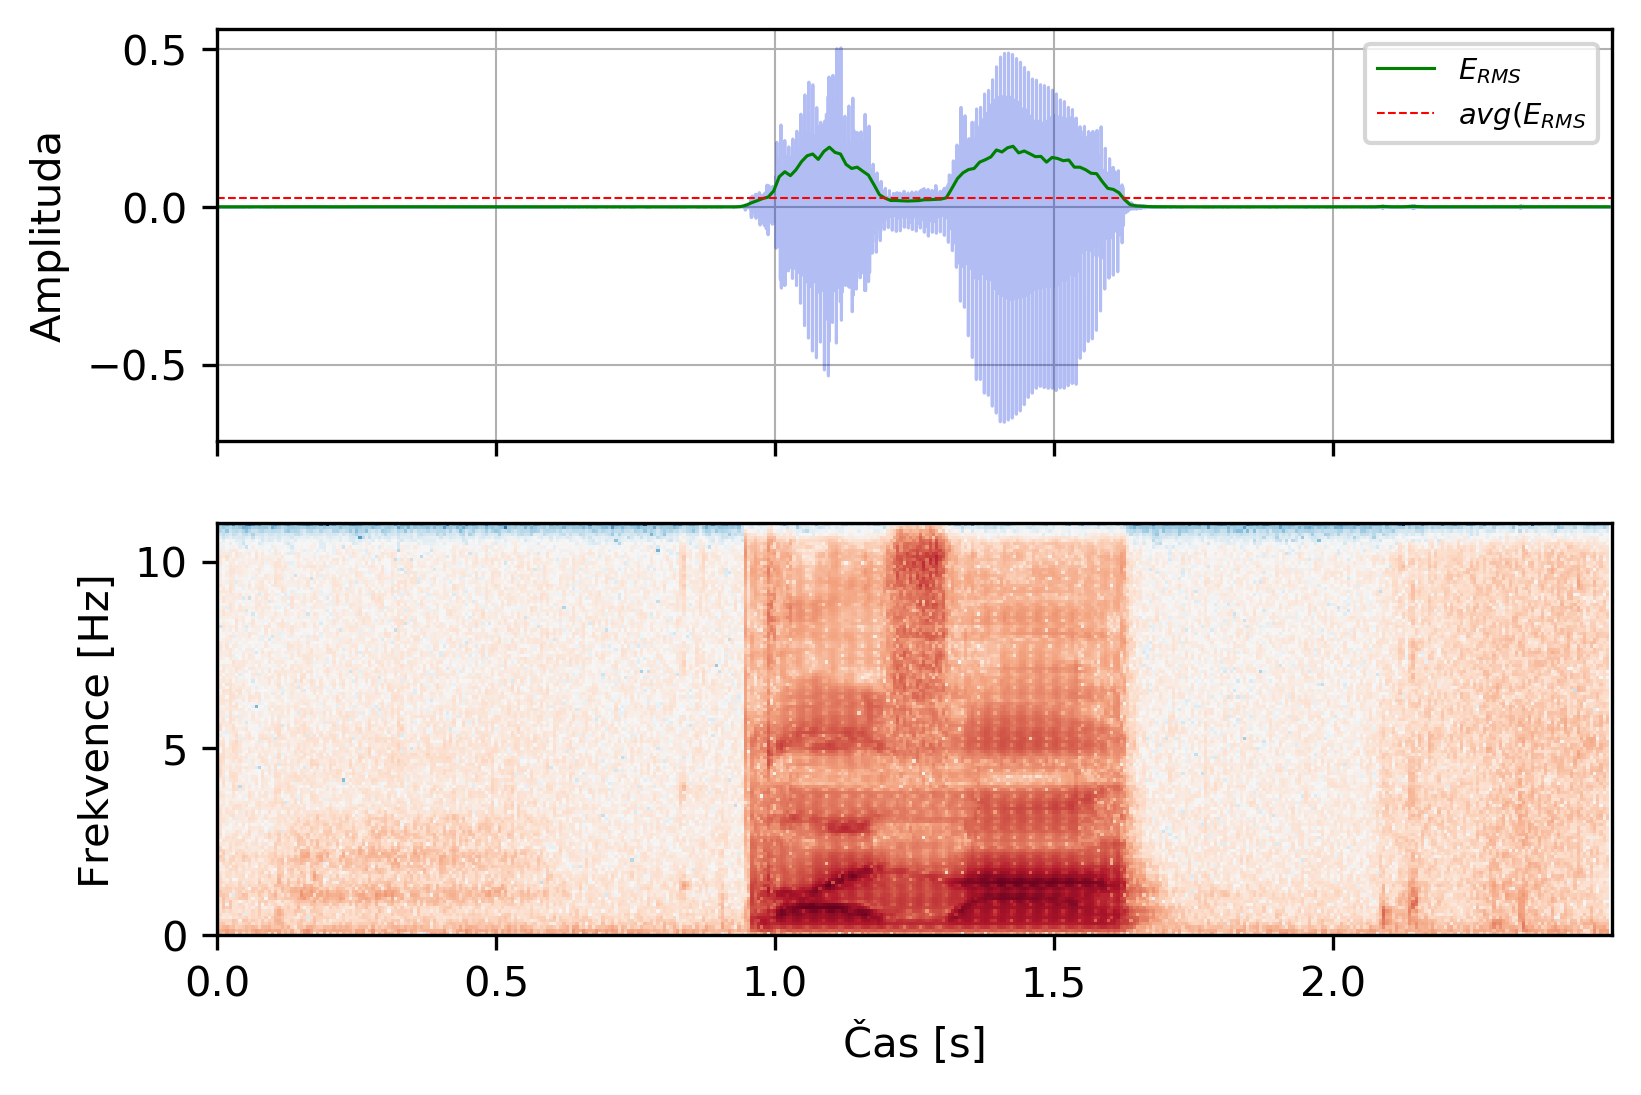
\includegraphics[width=0.9\textwidth]{./ch4-experiments/img/energy_spec_word.png}
  \caption{Průběh a spektrogram slova \uv{kosa} s společně s vyznačenou energií EL promluvy.}
  \label{fig:experiments:normalization:word}
\end{figure}

\begin{figure}[hbpt]
  \centering
  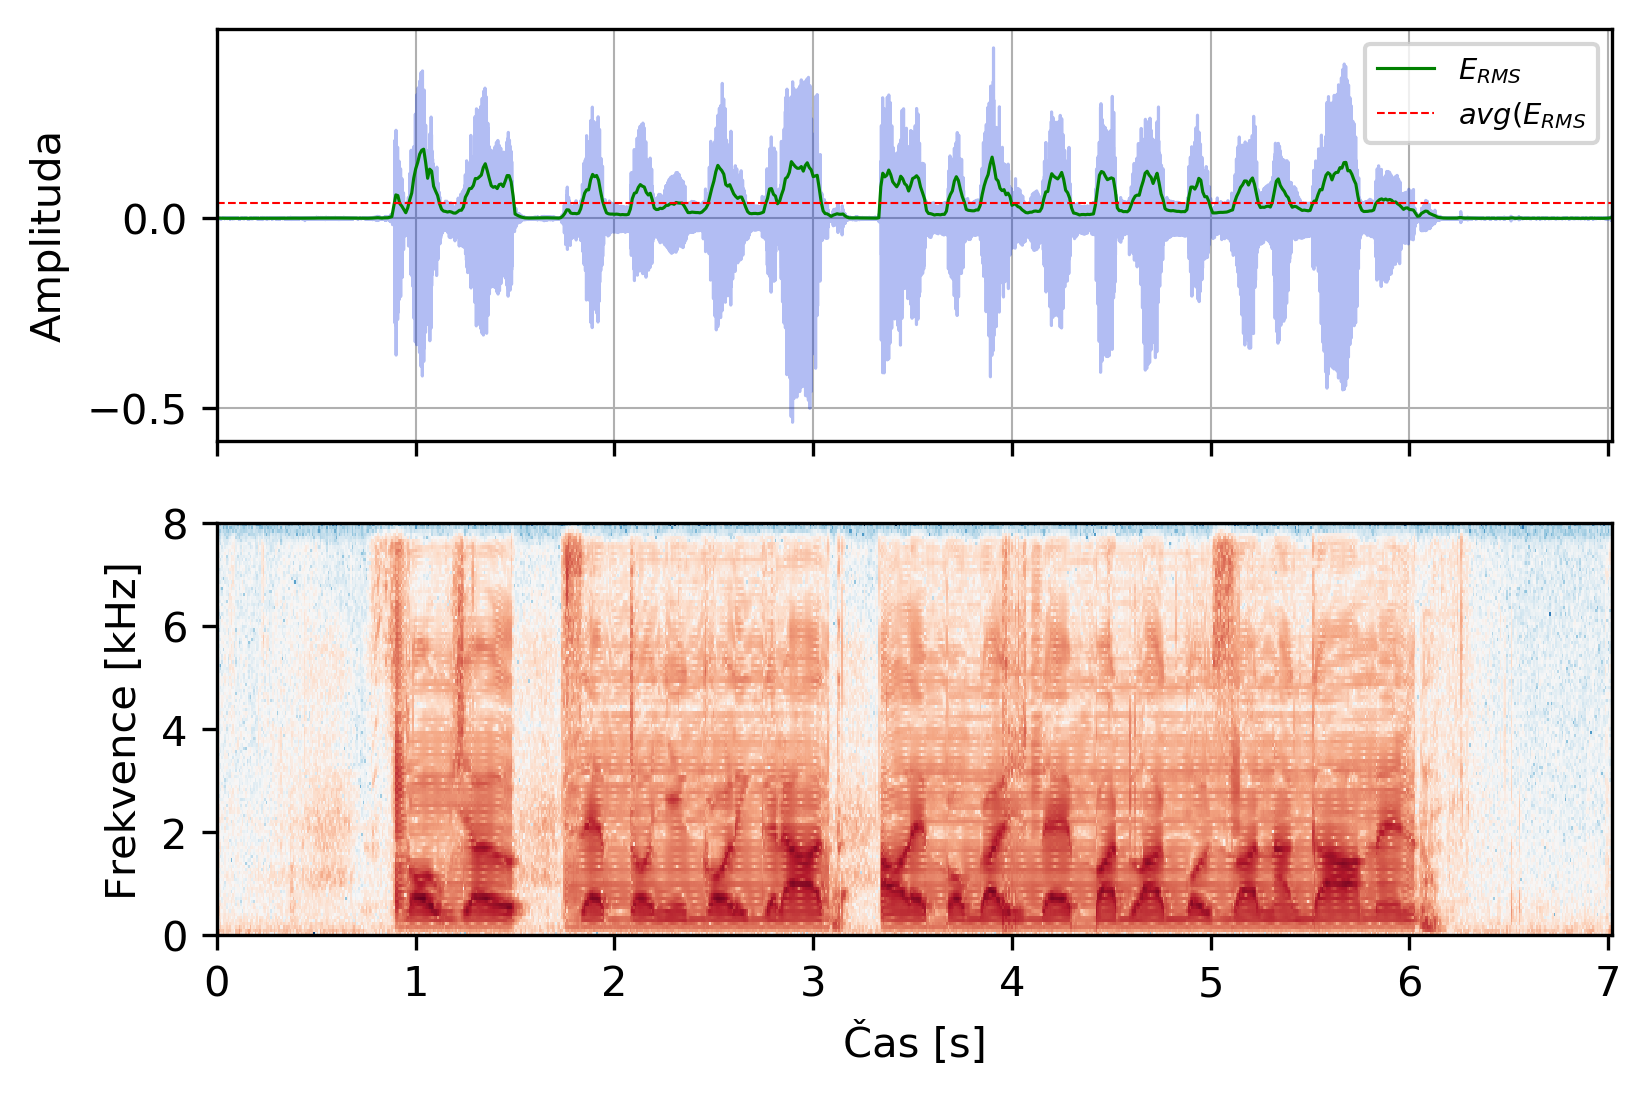
\includegraphics[width=0.9\textwidth]{./ch4-experiments/img/energy_spec_sentence.png}
  \caption{Průběh a spektrogram promluvy obsahující slovo \uv{kosa} a vyznačenou energií EL promluvy.}
  \label{fig:experiments:normalization:sentence}
\end{figure}

Tab. \ref{tab:experiments:normalization:recording} přibližuje souhrnné parametry nahrávek pořízených v 2. etapě nahrávání. Celkem se pořídilo přibližně 2 hodiny řeči (každá nahrávka obsahuje $0,5\ s$ ticha na začátku a konci). Z toho přibližně jen $10\ \%$ představují slova. Společně s novými daty tak korpus obsahuje téměř $14$ hodin audio záznamů a k nim příslušných přepisů.

\begin{table}[htpb]
  \centering
  \def\arraystretch{1.5}
  \pgfplotstabletypeset[
    col sep=comma,
    string type,
    columns/phase/.style={column name=Nahrávání, column type={|l}},
    columns/length/.style={column name=Délka \textit{[HH:MM:SS]}, column type={|r}},
    columns/words/.style={column name=Počet slov, column type={|r}},
    columns/sentences/.style={column name=Počet vět, column type={|r}},
    columns/files/.style={column name=Počet souborů, column type={|r|}},
    every head row/.style={after row=\hline, before row=\hline},
    every last row/.style={after row=\hline},
  ]{./ch4-experiments/tabs/0201-recording-stats.csv}
  \caption{Informace o korpusu nahrávek z 2. etapy nahravání.}
  \label{tab:experiments:normalization:recording}
\end{table}

\subsection{Vliv nových dat na kvalitu modelů}
\label{chap:experiments:normalization:quality}

Mezi lety 2012 a 2016 zaznamenalo rozpoznávání řeči překotný vývoj používaných technologií. Do té doby state-of-the-art modely stavěly na kombinaci HMM a \uv{gaussovských směsí} GMM. U těchto modelů má každý HMM stav jinou směs, viz obr. \ref{fig:experiments:normalization:hmm:gmm}. Pravděpodobnost přechodu mezi stavy HMM pak určují tyto směsi. Jejich parametry jsou získány na základě trénování. S příchodem open source frameworku Kaldi \cite{Kaldi2011} a rozmachem GPU výpočtů se začaly objevovat modely využívající hluboké neuronové sítě (DNN).

Rozpoznávání řeči je možné si představit sequence-to-sequence modely, tedy jako převod sekvence akustických parametrů do sekvence znaků/slov. Pro tento typ úloh se a priory hodí rekurentní neuronové sítě (RNN), ale jejich slabinou je enormní výpočetní náročnost i mimo trénovací fázi a také potřeba enormního množství dat, pokud má být vytvořen end-to-end\footnote{End-to-end systémem je ve valné většině případů myšlen systém, do kterého vstupuje audio framů a  vystupuje z něj sekvence znaků. Vyvojář takového systému často nepoužívá parametrizované audio.} systém \cite{Hannun2014}. Vytvoření čistě RNN end-to-end ASR systému je nesmírně nákladné (data, HW, atd.), tak se v současné době převážně využívá kombinace HMM modelu, který je také zástupcem rodiny sequence-to-sequence modelů, a DNN. Hlavním rozdílem oproti modelům s GMM je v tom, že pro všechny stavy HMM se trénuje pouze jedna neuronová síť, pomocí které jsou určovány přechody mezi stavy, viz obr. \ref{fig:experiments:normalization:hmm:dnn}. Navíc tím, že tato neuronová síť určuje \uv{pouze} přechody mezi jednitlivými stavy HMM, tak může být tato síť řádově menší a jednodušší, než kdyby se jednalo o end-to-end neuronovou síť. Tím pádem je rychleji natrénovaná a je potřeba řádově méně dat.


\begin{figure}[htpb]
  \centering
  \begin{subfigure}[b]{0.4\textwidth}
    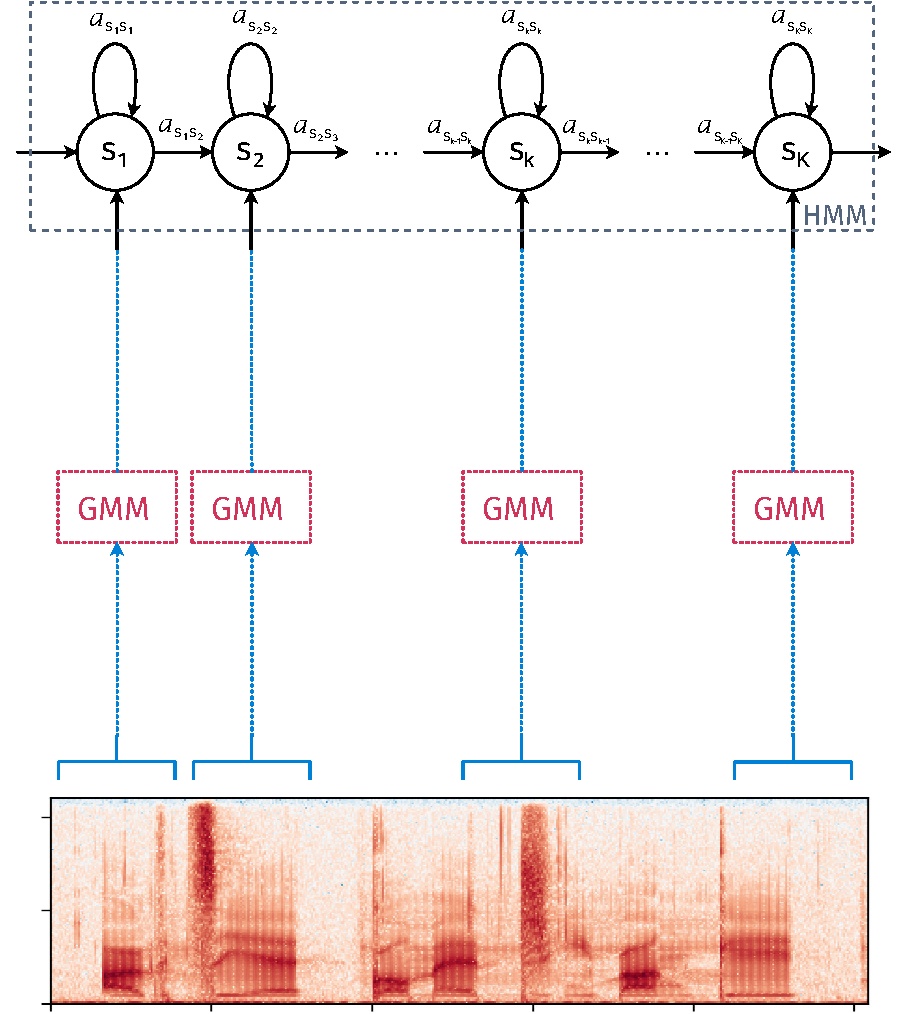
\includegraphics[width=\textwidth]{./ch4-experiments/img/gmm-hmm.pdf}
    \caption{GMM-HMM}
    \label{fig:experiments:normalization:hmm:gmm}
  \end{subfigure}
  %
  \begin{subfigure}[b]{0.4\textwidth}
    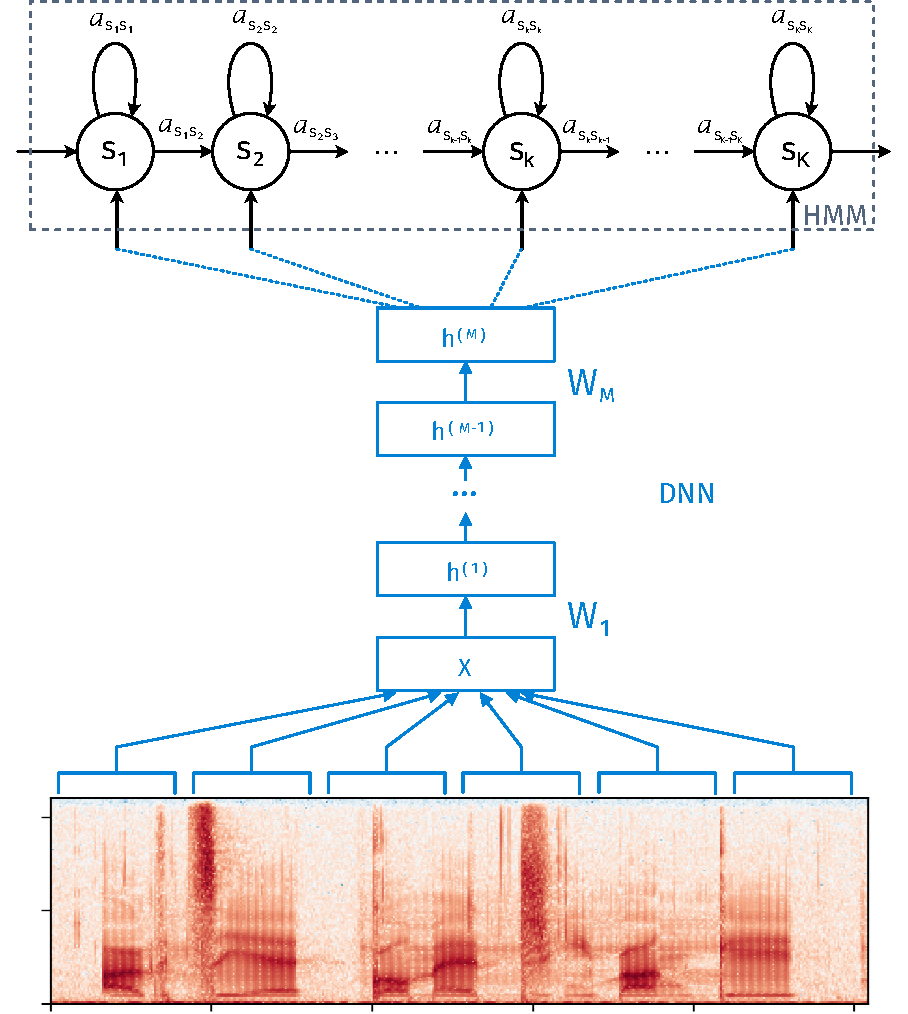
\includegraphics[width=\textwidth]{./ch4-experiments/img/dnn-hmm.pdf}
    \caption{DNN-HMM}
    \label{fig:experiments:normalization:hmm:dnn}
  \end{subfigure}
  \caption{Znázornění odlišného principu \textit{GMM-HMM} a \textit{DNN-HMM}.}
  \label{fig:experiments:normalization:hmm}
\end{figure}

\subsubsection{Ověření přínosu nových dat}

S novými daty je možné natrénovat modely a ověřit, zda je s nimi systém schopen pracovat. Oproti \ref{chap:experiments:analysis:experiment} je použit framework Kaldi, který se stal standardem pro vytváření akustikých modelů. Samotný framework se skládá z velkého množství utilit, která každá plní určitý \uv{jednoduchý} úkol v procesu vytváření/testování modelu. Kompletní proces vytváření modelu se tak sestává z postupného spouštění těchto utilit v přesně definovaném pořadí. Autoři frameworku připravili nepřeberné množství skriptů, které slouží k vytvoření různých typů modelů. Všechny modely pro EL řeč vycházejí ze skriptů pro natrénování modelů z Wall Street Journal (WSJ) korpusu, který je nejčastěji požíván jako jakýsi benchmark ASR systémů. Skripty jsou jen drobně upraveny, aby výsledný model odpovídal EL doméně a bylo jej vůbec možné vytvořit.

Přestože DNN nahradily GMM v HMM, tak k jejich natrénování je nezbytné nejprve natrénovat \textit{GMM-HMM} model, který slouží k prvotnímu zarovnání (určení hranic jednotlivých fonémů v rámci audio náhrávky). Toto zarovnání slouží jako startovní bod pro neuronovou síť. Tím, že je trénována pouze jedna síť, tak je k dispozici řádově více dat\footnote{V případě \textit{GMM-HMM} má každý stav své GMM a tím pádem, čím více stavů, tím méně trénovacích dat pro každou směs.} k jejímu natrénování, na druhou stranu má tato síť mnohem více parametrů než všechny GMM směsi dohromady a tak je potřeba dbát na velikost sítě. Nicméně pro standardní WSJ DNN (6 vrstev, každá s 1024, 2048 nebo 4096 neurony) je dat dostatek.

Přestože vývoj výpočetních GPU postupuje závratnou rychlostí, tak natrénování standardního \textit{DNN-HMM} modelu trvá o poznání déle než \textit{GMM-HMM}. Pro ověření zda je možné vytvořit model ze všech dat, která jsou k dispozici, poslouží i \textit{GMM-HMM} model, teb navíc slouží jako startovní bod pro \textit{DNN-HMM}, tak by se vytvářel tak jako tak. Pokud tyto modely neposkytnou DNN, alespoň trochu \uv{dobré} počáteční podmínky, tak sofistikovanější DNN nemusí pomoci.

Pro potřeby ověřovacího experimentu posloužily jako základ Kaldi WSJ skripty. Jako první je vytvořen monofónový akustický model používající Perceptual Linear Prediction (PLP) s 12 kepstrálními, delta a delta-delta koeficienty. Tento monofónový model je speciální případ kontextově závislých modelů, bez levého a pravého (fonémového) kontextu. Následně jsou natrénovány trifónové modely. Stejně jako v experimentech provedených v části \ref{chap:experiments:analysis:experiment}, tak i zde jsou použity rozhodovací stromy, protože počet všech variant trifónů je příliš velký.

V části \ref{chap:experiments:analysis:experiment} byl korpus rozdělen na trénovací a testovací sadu. Po rozšíření korpusu je rozdělení dat z 1. etapy ponecháno a nová data rozdělena mezi trénovací a testovací sadu. Všechny nahrané věty v 2. etapě jsou použity v trénovací a všechna slova naopak v testovací sadě. Toto rozdělení je logické, protože důvodem rozšíření korpusu je snaha ověřit funkčnost ASR systémů na slovech, která mají odlišný význam, ale liší se pouze znělostí jednoho fonému. Jelikož z výsledků v části \ref{chap:experiments:analysis:reduction} vyplývá, že určité spektrum trifónů je možné reprezentovat pouze pomocí znělých variant, tak při použití nahraných slov bude teoreticky možné lépe prozkoumat tuto otázku.

Pro otestování výše popsaného modelu je opět použit monofónový zerogramový jazykový model tak, aby co nejméně ovlivňoval dosažené výsledky. Na kompletní testovací sadě byla dosažena přesnost $54,96\ \%$. V případě, že testovací sada obsahovuje pouze nově nahraná slova, tak dokonce jen $42,97\ \%$. Což je významné zhoršení oproti výsledkům dosažených v \ref{chap:experiments:analysis:experiment}, kde bylo dosaženo více něž $80\ \%$ přesnosti. Pro výpočet přesnosti je ve všech případech použita rovnice \ref{eq:experiments:analysis:experiment:accuracy}.

Pro ověření, že není chyba v procesu trénování (přeci jen se změnil framework) poslouží křížový test, kdy pomocí stejného procesu jsou natrénovány modely z původních (1. etapa) a nových (2. etapa) dat a křížově otestovány na kompletní, původní a jen nové části testovací sady. Výsledky tohoto testu jsou v tab. \ref{tab:experiments:normalization:cross}. Z té je jasně patrné, že pokud je model natrénován a otestován pomocí dat pocházející ze stejné etapy, tak je dosaženo podobných výsledků jako v \ref{chap:experiments:analysis:experiment}. Trénovcací proces je tedy \uv{správný}.

%model;orig;new

\begin{table}[htpb]
  \centering
  \def\arraystretch{1.5}
  \pgfplotstabletypeset[
    col sep=semicolon,
    string type,
    columns/model/.style={column name=Model, column type={|c}},
    columns/orig/.style={column name=1. etata $[\%]$, column type={|r}},
    columns/new/.style={column name=2. etapa $[\%]$, column type={|r|}},
    every head row/.style={before row={
      \hline
      & \multicolumn{2}{c|}{Accuracy} \\
    },after row=\hline},
    every last row/.style={after row=\hline},
  ]{./ch4-experiments/tabs/0202-cross_test.csv}
  \caption{Křížový test modelů natrénovaných a otestovaných na datech z 1. a 2. etapy.}
  \label{tab:experiments:normalization:cross}
\end{table}

% - 20161208_param -> porovnani n vs o, vzit hodnoty z toho
% - 20170111_together -> CMN FULL vysledky na HMM, pak tam dat i vysledky z

\subsubsection{Eliminace vlivu kanálu}

Z dosažených výsledků tedy vyplývá, že nová data jsou příliš odlišná od původních a v parametrickém prostoru příliš vzdálena těm původním. Zároveň je těchto dat relativně malé množství, aby se mohly modely plně adaptovat. Na rozdíl v datech se můžeme koukat jako na změnu kanálu, která je příčinou těchto změn. Řečník je přeci stejný. V předchozím textu bylo zmíněno, že v rámci 2. etapy došlo ke změné nahrávací procedury a také elektrolarynxu. Tím byl pozměněn kanál a logicky výsledná zaznamenaná řeč má jiné parametry než ta v 1. etapě. Mezi další prvky, které mohou způsobit změnu kanálu může být prostředí, tedy jestli je řeč produkována uvnitř nějaké místnosti, či venku, jestli je na pozadí přítomen šum atd. K tomu, aby bylo možné použít všechna dostupná data, je potřeba eliminovat tento vliv kanálu. K jeho eliminaci je možné využít CMN, což je zkratka anglických slov Cepstral Mean Normalisation. Principem této metody je odstranení vlivu kanálu na základě střední hodnoty kepstrálních koeficientů, viz dále.

Zaznamenaný signál je možné popsat jako konvoluci promluvy a řeči, matematicky zapsáno jako

\begin{equation}
  y\left[n\right] = x\left[n\right] \circledast h\left[n\right],
  \label{eq:experiments:normalization:convolution}
\end{equation}

\noindent kde $x\left[n\right]$ představuje vstupní signál, tedy řeč, a $h\left[n\right]$ odezvu kanálu na jednotkový impulz. Zaznamenaný signál je jejich již zmíněnou lineární konvolucí. Ve frekvenční oblasti je pak rovnice \ref{eq:experiments:normalization:convolution} zapsaná následovně:

\begin{equation}
  Y\left[f\right] = X\left[f\right] \cdot H\left[f\right]
\end{equation}

\noindent V této oblasti se z konvuluce stalo násobění, což značně zjednodušuje situaci. K odstranění vlivu kanálu je, ale ještě potřeba převést hodnoty do kepstrálná oblasti. To je realizováno pomocí logaritmu spektra

\begin{equation}
  Y\left[q\right] = \log\left(Y\left[f\right]\right) = \log\left(X\left[f\right] \cdot H\left[f\right]\right) = X\left[q\right] + H\left[q\right],
\end{equation}

\noindent kde $q$ představuje kepstrální koeficient. V kepstrální oblasti je vliv kanálu aditivní složkou výsledného záznamu. Problémem však je, že konkrétní hodnota vlivu kanálu je neznáma, protože k dispozici je pouze výsledný ovlivněný signál. Předpokládejme však, že vliv kanálu je stacionární\footnote{Jedná se sice o silný, ale logický předpoklad. Pokud se vztáhne k pořízenému řečovému korpusu, tak v rámci jedné etapy nahrávání, je proces nahrávání neměnný, tzn. je použita stejná aparatura a k nahrávání dochází vždy ve stejné místnosti.}, tak poté je možné každý frame nahrávky $i$ zapsat jako

\begin{equation}
  Y_i\left[q\right] = H\left[q\right] + X_i\left[q\right],
\end{equation}

\noindent kde $Y_i\left[q\right]$ představuje $i$ frame kepstra $q$ nahrávky a $X_i\left[q\right]$ představuje $i$ frame kepstra $q$ neovlivněné řeči. Z této rovnice je pak možné vypočítat střední hodnotu

\begin{equation}
  \frac{1}{N} \sum_i Y_i\left[q\right] = H\left[q\right] + \frac{1}{N} \sum_i X_i\left[q\right].
\end{equation}

\noindent Vliv kanálu je pak možné eliminovat odečtením střední hodnoty kepstra $q$ od aktuální hodnoty kepstra $Y_i\left[q\right]$

\begin{align}
  R_i\left[q\right] &= Y_i\left[q\right] - \dfrac{1}{N}\sum_{j} Y_j\left[q\right] \nonumber  \\
  &= H\left[q\right] + X_i\left[q\right] - \left( H\left[q\right] + \frac{1}{N} \sum_j X_j\left[q\right] \right) \nonumber  \\
  &= X_i\left[q\right] - \frac{1}{N} \sum_j X_j\left[q\right]
  \label{eq:experiments:normalization:cmn}
\end{align}

\noindent S pomocí rovnice \ref{eq:experiments:normalization:cmn} je možné odfiltrovat vliv kanálu a teoreticky tak získat hodnoty kepstrálních koeficientů odpovídající nezkreslené řeči. Otázkou je, přes jaký úsek počítat střední hodnotu. Je možné ji počítat přes posuvné okénko fixní délky, přes jednotlivé nahrávky, nebo dokonce přes všechny nahrávky konkrétní etapy. Pokud totiž bude úsek, přes který je počítána průměrná hodnota, krátký, tak se může stát, že vypočtená střední hodnota nebude odpovídat skutečné střední hodnotě umožňující eliminaci vlivu kanálu. V tomto případě, kdy nahrávky dělí velký časový úsek a i proces nahrávání byl změněn, je toto potřeba odexperimentovat.

Pro zjištění jaká možnost je optimální je použit stejná trénovací procesdura jako v předešlých experimentech s novými daty. Jediný rozdíl je v datech na kterých bylo aplikováno CMN. Celkem byly uvažovány dva experimenty, a to

\begin{itemize}
  \item CMN počítáno pro každou nahrávku,
  \item CMN počítáno pro celou etapu,
\end{itemize}

\noindent algoritmus CMN implementovaný na datech byl implementován na katedře kybernetiky Fakulty aplikovaných věd.

V tab. \ref{tab:experiments:normalization:cmn:file} jsou výsledky experimentu s cmn počítaném přes jednotlivé nahrávky. Z dosažených výsledků je zřejmé, že pokud se CMN počítá přes jednotlivé nahrávky, tak je oproti výsledkům v tab. \ref{tab:experiments:normalization:cross} dosaženo určitého zlepšení, zvláště pokud je model natrénován na datech z 1. etapy a otestován na datech z 2. etapy, ale výsledky nejsou zdaleka tak dobré, jako v případě, že je model natrénován a otestován na datech ze stejné sady. Vliv tu také může hrát fakt, že zejména nahrávky izovlovaných slov jsou relativně krátké a vypočtené střední hodnoty, tak nabývají odličných hodnot.

\begin{table}[htpb]
  \centering
  \def\arraystretch{1.5}
  \pgfplotstabletypeset[
    col sep=semicolon,
    string type,
    columns/model/.style={column name=Model, column type={|c}},
    columns/orig/.style={column name=1. etata $[\%]$, column type={|r}},
    columns/new/.style={column name=2. etapa $[\%]$, column type={|r|}},
    every head row/.style={before row={
      \hline
      & \multicolumn{2}{c|}{Accuracy} \\
    },after row=\hline},
    every last row/.style={after row=\hline},
  ]{./ch4-experiments/tabs/0203-cmn_file.csv}
  \caption{Křížový test modelů natrénovaných a otestovaných na datech z 1. a 2. etapy s CMN přes jednotlivé soubory.}
  \label{tab:experiments:normalization:cmn:file}
\end{table}

Dalším experimentem tedy je s daty, kde bylo CMN vypočteno ze všech nahrávek konkrétní etapy. V tab. \ref{tab:experiments:normalization:cmn:full} je vydět markantní zlepšení výsledků. Pokud byl model natrénován na datech z 1. etapy a test byl proveden na datech z libovolné etapy, tak dosažené výsledky jsou velmi podobné. Nejhoršího výsledku je dosaženo, pokud je model natrénován na datech z 2. etapy a otestován na těch z té 1. V tomto případě hraje velký vliv, že model je natrénován z relativně malého množství dat (pouhé 2 hodiny). Pokud je tedy CMN počítáno přes všechny nahrávky v etapě, tak je dosaženo významného zlepšení a vlivk kanálu je v podstatě eliminován. Pro doplnění je dobré zmínit, že pokud je model natrénován ze všech trénovacích dat (1. a 2. etapa) a otestován pomocí kompletní testovací sady, tak je dosažená přesnost s monofónovým zerogramovým jazykovým modelem rovna $77,69\ \%$, což je výsledek přibližující se hodnotám dosaženým v prvnotních experimentech v části \ref{chap:experiments:analysis:experiment}.

\begin{table}[htpb]
  \centering
  \def\arraystretch{1.5}
  \pgfplotstabletypeset[
    col sep=semicolon,
    string type,
    columns/model/.style={column name=Model, column type={|c}},
    columns/orig/.style={column name=1. etata $[\%]$, column type={|r}},
    columns/new/.style={column name=2. etapa $[\%]$, column type={|r|}},
    every head row/.style={before row={
      \hline
      & \multicolumn{2}{c|}{Accuracy} \\
    },after row=\hline},
    every last row/.style={after row=\hline},
  ]{./ch4-experiments/tabs/0204-cmn_full.csv}
  \caption{Křížový test modelů natrénovaných a otestovaných na datech z 1. a 2. etapy s CMN přes všechny nahrávky v etapě.}
  \label{tab:experiments:normalization:cmn:full}
\end{table}

Z výsledků v tab. \ref{tab:experiments:normalization:cmn:file} je možné odvodit, že pokud se CMN počítá přes posuvné okénko fixní délky, tak dosažené výsledky nejsou zrovna dobré. Což se i experimentálně potvrdilo, když výsledná přesnost dosáhla hodnoty $56,51\ \%$, pokud jsou použita všechna data. Nicméně framefork Kaldi umožňuje aplikování CMVN, což je Cepstral mean and variance normalization. Oproti standardními CMN je uvažována i variance v kepstrální oblasti. Technicky je pravá část rovnice \ref{eq:experiments:normalization:cmn} ještě podělena vypočtenou variancí daného kepstrálního koeficientu $q$. Takže pokud je použito Kaldi CMVN, tak výsledná přesnost, na modelu trénovaném a testovaném na všech datech, dosáhla hodnoty $76,15\ \%$. Tento výsledek je srovnatelný s modelem využívající CMN přes všechny nahrávky v dané etapě.

Po zjištění vhodného použití CMN pro odfiltrování vlivu kanálu je dalším krokem natrénování neuronové sítě. V předchozím textu bylo zmíněno, že neuronová síť jako počáteční podmínky používá zarovnání získané pomocí GMM. Počáteční zarovnání je získáno díky natrénovaným modelům s CMN přes všechny nahrávky. Trénovaná neuronová síť je typu fully connected feedforward síť s 6 vrstvami (5 skrytých vrstev). Postupně je natrénována síť s 1024, 2048 a 4096 neurony v každé vrstvě, výstupní vsrva je typu softmax s dimenzí rovnou počtu HMM stavů. Jazykový model je stejně jako u všech předchozím experimentů monofónový zerogramový. Tab. \ref{tab:experiments:normalization:dnn} ukazuje dosažené výsledky všech natrénovaných variant. Nejlepší přesnosti dosáhl model s 4096 neurony v každé vrstvě, ale rozdíl oproti ostatním variantám není velký. Oproti nejlepšímu GMM modelu DNN síť přidala dalších $6,97\ \%$ absolutně.

\begin{table}[htpb]
  \centering
  \def\arraystretch{1.5}
  \pgfplotstabletypeset[
    col sep=semicolon,
    string type,
    columns/neurons/.style={column name=Počet neuronů, column type={|c}},
    columns/accuracy/.style={column name=Accuracy $[\%]$, column type={|r|}},
    every head row/.style={before row=\hline,after row=\hline},
    every last row/.style={after row=\hline},
  ]{./ch4-experiments/tabs/0205-dnn.csv}
  \caption{Dosažená přesnost neuronové sítě s monofónovým zerogramovým jazykovám modelem.}
  \label{tab:experiments:normalization:dnn}
\end{table}

\subsection{Poslechový test}
\label{chap:experiments:normalization:listening}

V předchozím textu byly prezentovány různé dosažené výsledky, ale ty zatím nedokázali odpovědět na zásadní otázku: \uv{Dokáže se stroj\footnote{Stroj je zde reprezentován systémem automatického rozpoznávání řeči.} vyrovnat človéku?}. Přestože je EL řeč na první poslech obtížně srozumitelná, tak již po krátké době je člověk schopný obstojně poruzumnět. S přibývajícím časem se do určité míry porozumnéní ještě zlepšuje. Jak je na tom tedy stroj v porovnání s člověkem?

Ještě než je vůbec možné na tuto otázku odpovědět, tak je dobré si odpovědět na otázku: \uv{Jakým způsobem porovnat schopnosti člověka a stroje?}. K tomu může posloužit poslechový test, ve kterém mají posluchačí za úkol určit, z předem definovaných možností, co je obsahem promluv. Otestování schopností stroje pak probíhá pomocí experimentu, kde na vstupu systému jsou stejné promluvy, která jsou součástí poslechového testu, a výstupem je přepis. Metrika je pak počítána na základě správně/špatně určeného obsahu promluv. Prostým porovnáním správně určeného obsahu člověka a stroje je pak možné odpovědět na první \uv{položenou} otázku.

Při přípravě experimentu vykrystalizovaly tyto varianty poslechového testu:

\begin{itemize}
  \item test na izolovaných slovech,
  \item test na slovních bigramech.
\end{itemize}

\noindent Tím, že promluvy obsahují pouze izolovaná slovo (v druhém případě dvojici slov) je do značné míry eliminován vliv kontextu. Ten v mnohých případech pomáhá se správným určením významu slova i přesto, že nebylo dobře rozumnět. Pokud se bude navíc experiment skládat z množiny promluv, která obsahuje pouze slova popsaná v části \ref{chap:experiments:normalization:corpus}, tak je možné  určit jak \uv{dobře} je člověk (stroj) určit význam a případně od sebe odlišit tato slova.

\subsubsection{Izolovaná slova}

Určení významu slova, které bylo vysloveno v klidném prostředí se jeví jako velice jednoduchý úkol, ale pokud jej vyslovil řečník používající EL, tak už to tak snadné být nemusí, zvlášť pokud se jedná o slova v popsaná v \ref{chap:experiments:normalization:corpus}. V tomto případě mají účastníci poslechového testu za úkol postupně vyslechnout $320$ nahrávek izolovaných slov a vybrat jednu z předem definovaných odpovědí:

\begin{enumerate}[label=\alph*)]
  \item slovo A \textit{(např. kosa)},
  \item slovo B \textit{(např. koza)},
  \item nemohu rozhodnout.
\end{enumerate}

\noindent Ve výčtu možností je vždy skutečně pronesené slovo a k němu pak varianta lišící se pouze znělostí jednoho fonému. První dvě možnosti jsou vždy v abecedním pořadí. Nahrávky použité v rámci poslechového testu odpovídají nahraným slovům v rámci 2. etapy nahrávání. Poslechového testu se účastnilo $19$ subjektů z řad kolegů.

Výstupem poslechového testu je tabulka s procentuálním zastoupením jednotlivých odpovědí pro každou nahrávku. V tab. \ref{tab:experiments:normalization:isolated} je zobrazen výňatek získaných výsledků. Správné odpovědi jsou zvýrazněny tučně. První příklad reprezentuje situaci kdy účastník nebyl jednoznačně schopen určit význam slova. Druhý příklad pak ukazuje situaci, kdy všichni účastníci vybrali z komplementárních slov vždy pouze jediné, a to nehledě na to, které jim bylo ve skutečnosti puštěno. V tomto konkrétním případě tedy posluchači vždy \uv{slyšeli} slovo \uv{koza}. Dalo by se tedy usuzovat, že slova \uv{kosa} je akusticky identické se slovem \uv{koza}. Poslední případ reprezentuje situaci, kdy většina účastníků byla schopna určit správně význam slova. Celková přesnost pak dosáhla hodnoty $Acc_w^{human} = 70,47\ \%$ a byla vypočtena pomocí následujícího vzorce

\begin{equation}
  Acc_w^{human} = \frac{1}{n} \sum_{i=1}^{N} f_i * 100,
  \label{eq:experiments:normalization:accuracy:human}
\end{equation}

\noindent kde $n=320$ a $f_i$ se rovná relativní frekcenci správných odpovědí na otázku $i$ v poslechovém testu s izolovanými slovy.

\begin{table}[htpb]
  \centering
  \def\arraystretch{1.5}
  \pgfplotstabletypeset[
    col sep=semicolon,
    string type,
    columns/word/.style={column name=Slovo, column type={|l}},
    columns/option1/.style={column name=Možnost \textit{\textbf{a)} [\%]}, column type={|r}},
    columns/option2/.style={column name=Možnost \textit{\textbf{b)} [\%]}, column type={|r}},
    columns/option3/.style={column name=Možnost \textit{\textbf{c)} [\%]}, column type={|r|}},
    every head row/.style={after row=\hline, before row=\hline},
    every row no 1/.style={after row=\hline},
    every row no 3/.style={after row=\hline},
    every last row/.style={after row=\hline},
  ]{./ch4-experiments/tabs/0206-isolated.csv}
  \caption{Ukázka výsledku poslechového testu na izolovaných slovech.}
  \label{tab:experiments:normalization:isolated}
\end{table}

\subsubsection{Slovní bigramy}

V druhém poslechovém testu mají za úkol vyslechnout $333$ nahrávek slovních bigramů\footnote{Nahrávky obsahují dvě po sobě vyslovená slova.} a vybrat jednu z předem definovaných odpovědí. Ty mají vždy následující formát

\begin{enumerate}[label=\alph*)]
  \item slovo A + slovo A \textit{(např. kosa + kosa)},
  \item slovo A + slovo B \textit{(např. kosa + koza)},
  \item slovo B + slovo A \textit{(např. koza + kosa)},
  \item slovo B + slovo B \textit{(např. koza + koza)}.
\end{enumerate}

\noindent Je zřejmé, že to představuje všechny kombinace, které lze z dvojice vytvořit. Dvojice slov vždy tvoří již několikrát zmíněné dvojice slov mající jiný význam, ale lišící se právě v jednom fonému. Rozšířený řečový korpus, tak jak je popsaný v části \ref{chap:experiments:normalization:corpus}, ale neobsahuje tento typ nahrávek. Tím pádem je potřeba je vytvořit \uv{uměle}. Což není velký problém, protože každá nahrávka izolovaného slova obsahuje minimálně $0,5\ s$ ticha na začátku a konci. Pokud jsou tyto nahrávky spojeny\footnote{Ke spojení je možné použít nástroj \textit{ffmpeg} nebo \textit{sox}.}, vznikne jediná nahrávka obsahující dvě zájmová slova oddělena krátkou pauzou. Z každé dvojice slov vznikly vždy dvě nahrávky lišící se pořadím slov.

Vyšší počet položek v testu je zapříčiněn faktem, že pro určitá slova existuje více než jedna kombinace s jiným slovem\footnote{Ve valné většině se jedná o slova obsahující písmena \textit{i/y}, která jsou v akustické formě identická. Příkladem může být dvojice \textit{nebyli + nepili} a \textit{nebili + nepili}.}. Ve snaze zkrátit, už tak docela náročený poslechový test, byly vygenerovány bigramy odpovídající poiuze možnostem \textit{b)} a \textit{c)}. Účastníci poslechového testu o tom však nebyli informováni. Přesto tento poslechový test dokončilo pouze $12$ účastníků.

Stejně jako u testu s izolovanými slovy je výstupem testu tabulka obsahující procentuální zastoupení jednotlivých odpovědí na každou otázku. Tab. \ref{tab:experiments:normalization:bigrams} obsahuje ukázku těchto výsledků. Stejně jako v předchozím případě, správné odpovědi jsou zvýrazněny tučně. Ačkoli jsou nyní v testu dvojice slov, tak dosažené výsledky do značné míry korespondují s výsledky z testu s izolovanými slovy (viz tab. \ref{tab:experiments:normalization:isolated}). V prvním případě (\textit{borci + porci}) nebyli účastníci schopni jednoznačně určit význam slov v nahrávce, stejně jako v případě testu na izolovaných slovech. V druhém případě (\textit{kosa + koza}) všichni posluchači až na jednoho vybrali možnost \textit{d)}, tedy \textit{koza + koza}. Správný výběr jedním účastníkem lze považovat spíše za náhodu, protože v případě opačného pořadí slov již nikdo správnou odpověď nevybral. Je dobré zmínit, že účastníci v žádném poslechovém testu nebyli omezeni v počtu opětovného přehrání promluvy. Tím pádem je velmi pravděpodobné, že tento konrétní participant opakovaně poslouchal danou nahrávku a hledal rozdíl až nějaký drobný zaznamenal. Otazkou však je jestli to spíš nebyla sugesce a to již zmíněné štěstí.

Poslední prezentovaný příklad zastupuje množinu odpovědí, kdy účastníci naprosto správně určili význam slov. Průměrná dosažená přesnost člověka, počítána pomocí rovnice \ref{eq:experiments:normalization:accuracy:human}, dosáhla hodnoty $Acc_{p}^{human} = 66,24\ \%$.

\begin{table}[htpb]
  \centering
  \def\arraystretch{1.5}
  \pgfplotstabletypeset[
    col sep=semicolon,
    string type,
    columns/word/.style={column name=Slovní bigram, column type={|l}},
    columns/option1/.style={column name=Mož. \textit{\textbf{a)} [\%]}, column type={|r}},
    columns/option2/.style={column name=Mož. \textit{\textbf{b)} [\%]}, column type={|r}},
    columns/option3/.style={column name=Mož. \textit{\textbf{c)} [\%]}, column type={|r}},
    columns/option4/.style={column name=Mož. \textit{\textbf{d)} [\%]}, column type={|r|}},
    every head row/.style={after row=\hline, before row=\hline},
    every row no 1/.style={after row=\hline},
    every row no 3/.style={after row=\hline},
    every last row/.style={after row=\hline},
  ]{./ch4-experiments/tabs/0207-bigrams.csv}
  \caption{Ukázka výsledku poslechového testu na dvojicích slov.}
  \label{tab:experiments:normalization:bigrams}
\end{table}

\subsection{Výsledky porovnání}
\label{chap:experiments:normalization:comparison}

Výsledky poslechového testu ukázaly jak je na tom člověk. Nyní je potřeba zjistit jak je na tom vlastně stroj. K tomu je nezbytné natrénovat akustický model a použít vhodný jazykový model. Jako akustický model je použitá neuronová síť popsaná v části \ref{chap:experiments:normalization:quality}. Jedná se tedy o DNN s $6$ vrstvami ($5$ skrytých vrstev, každá s $4096$ neurony), výstupní vrstva je typu softmax s dimenzí rovnou počtu HMM stavů. Jako parametrizace je použito PLP (statické + delta + delta-delta parametry) a pro eliminaci vlivu kanálu pak CMN. Výsledný příznakový vektor má dimenzi $40$ (viz část \ref{chap:experiments:analysis:reduction}). Vstupem neuronové sítě je pak parametrizované okénko mající kontext přes $5$ framů\footnote{Celkem je $5$ framů předchazející a $5$ následující aktuální frame.}. Vstupní dimenze neuronové sítě je tedy $440$. K natrénování takovéhoto modelu je použit framework Kaldi. Oproti dosavadním experimentům je v tomto případě použit vlastní real-time dekodér. Tento LVCSR systém je optimalizován pro co nejnižší latenci a je schopný pracovat velmi velkými slovníky, čítající miliony položek. Tento dekodér byl vyvinut na katedře kybernetiky Fakulty aplikovaných věd.

Z poslechových testů jsou k dispozici dva výsledky. První reprezentuje schopnost určit význam izolovaného slova. Druhý pak schopnost od sebe rozeznat dvě velmi podobná slova. Pro potřeby porovnat tyto výsledky s těmi dosaženými ASR systémem jsou vytvořeny celkem $3$ experimenty využívající výše popsaný Kaldi model.

První experiment odpovídá poslechovému testu s izolovanými slovy a jeho základem je zerogramový LM obsahující více než 1 milion slov. Většina předchozích experimentů využívala monofónový zerogramový model, aby bylo možné eliminovat jeho vliv na výsledné přesnosti. U těchto experimentů je, ale tento LM nevyhovující, protože cílem je správně rozpoznat celé slovo, a proto je využit slovní jazykový model. U zerogramového modelu mají všechny položky stejnou pravděpodobnost, tím je zaručeno, že nebudou preferována četnější slova. Data pro tento LM pocházejí z novinových článků, webových zpravodajských serverů, filmových titlků a přepisů televizních pořadů. Využití takto velkého LM vychází z představy, že i člověk má velkou slovní zásobu a dopředu neví co bude obsahem konkrétní promluvy v rámci testu. Tento test je pojmenován jako \uv{onemil}.

Ve skutečnosti však, v rámci poslechového testu, účastníci znají seznam slov zahrnutých do testu a mají tak určitou výhodu oproti \uv{onemil} nastavení. Ke kompenzaci tohoto faktu, je vytvořen druhý experiment, který má redukovaný LM. Ten obsahuje pouze slova, která se opravdu vyskytla v rámci poslechového testu. Tento experiment je nazván jako \uv{reduced}. Výsledky obou těchto experimentů jsou porovnány s poslechovým testem na izolovaných slovech. Další možností by mohlo být vytvoření speciálních LM pro každou promluvu obsahující pouze komplementární slova. Bohužel problémem je, že poslechový test obsahuje ještě 3 možnost (\uv{nemohu rozhodnout}) a v případě, že by LM obsahoval pouze dvě slova, tak by ASR experiment, svými parametry, neodpovídal poslechovému testu.

Poslední experiment odpovídá druhému poslechovému testu. K získání srovnatelných výsledků, je pro každý slovní bigram vygenerován speciální zerogramový LM. Ten obsahuje vždy pouze všechny 4 kombinace slov. Tím pádem odpovídá dostupným možnostem v rámci druhého poslechového testu. Tento experiment je nazván jako \uv{bigrams} a jeho výsledky jsou porovnány s druhým poslechovým testem.

Výsledkem rozpoznávače je nejlepší hypotéza (případně \textit{N} nejlepších hypotéz), tudíž slovo. To však není porovnatelné s výsledkem poslechového testu. Z tohoto důvodu jsou všechny výsledky systému ASR ohodnoceny $1$, pokud bylo výstupem správné slova, v opačném případě pak $0$. Násladně byl z tohoto ohodnocení vypočten průměr. Pro upřesnějí je nutné zmínit, že \textit{i/y} na výsledném ohodnocení nehraje roli. Dosažené výsledky jsou pak v tab. \ref{tab:experiments:normalization:comparison}. Ty ukazují, že požedovaný úkol je výzvou i pro samotného člověka, natož pro stroj. V případě experimentu \uv{onemil} je výkon ASR systému významně horší než výkon člověka. To je zejména způsobeno enormní perplexitou jazykového modelu. Ta je přímo rovna velikosti slovníku. Zmenšením slovníku se podařilo získat výsledky srovnatelné s člověkem. Je dobré zdůraznit, že i v případě \uv{reduced} experimentu hrají karty ve prospěch člověka, protože čelí pouze perplexitě $3$, protože se kdykoli může podívat na nabízené možnosti. Řešením by bylo nechat účastníky přepsat obsah promluvy a porovnat ho se skutečným obsahem. Nicméně toto by významně zvýšílo náročnost (zejména časovou) poslechového testu a bylo by velmi komplivané získat kompletní výsledky od relevantního množství účastníků. Už jen podíl odpadlíků mezi prvním a druhým poslechovým testem činil závratných $30\ \%$.

Velmi zajímavé jsou výsledky u \uv{bigrams} experimentu. Na první pohled se může jevit jako snazší, protože úkolem je vybrat z jasně definovaných kombinací slov. Avšak slova jsou si akusticky velmi podobná a v mnoha případech je velmi náročné je od sebe rozeznat. Jak člověk, tak stroj, dosáhli v tomto testu nejhorších výsledků. Při analýze se ukázalo, že rozdíly mezi hypotézami ASR systému jsou velmi malé, což naznačuje velkou podobnost mezi inkriminovanými modely fonémů. Zároveň tyto výsledky s velmi podobnými hypotézami korelují s výsledky poslechového testu, kde posluchači nebyli schopni jednoznačně rozhodnout o významu jednotlivých slov.

\begin{table}[htpb]
  \centering
  \def\arraystretch{1.5}
  \pgfplotstabletypeset[
    col sep=semicolon,
    string type,
    columns/type/.style={column name= , column type={|l}},
    columns/onemil/.style={column name=onemil \textit{[\%]}, column type={|r}},
    columns/reduced/.style={column name=reduced \textit{[\%]}, column type={|r}},
    columns/bigrams/.style={column name=bigrams \textit{[\%]}, column type={|r|}},
    every head row/.style={after row=\hline, before row=\hline},
    every last row/.style={after row=\hline},
  ]{./ch4-experiments/tabs/0208-comparison.csv}
  \caption{Porovnání dosažených výsledků člověka a stroje.}
  \label{tab:experiments:normalization:comparison}
\end{table}

Z dosažených výsledků je zřejmé, že stroj nedosahuje schopností člověka. Pokud se vezme v úvahu, že byl člověk oproti stroji vždy v malé výhodě, tak dosažené výsledky jsou relativně optimistické, protože minimálně v jednom případě se stroj téměř vyrovnal člověku. Samotnou kapitolou je vliv kontextu. Ještě před samotnými ASR experimenty byl ověřen výkon ASR systému na \uv{kontinuální} řeči, zde reprezentované větami z testovací sady. Jazykovým modelem je v tomto případě trigramový model obsahující $1,2$ milionu unikátních slov. Přesnost na slovech (počítaná pomocí rovnice \ref{eq:experiments:analysis:experiment:accuracy}) dosáhla hodnoty $86,10\ \%$. Při porovnání s výsledky z tab. \ref{tab:experiments:normalization:comparison} jasně plyne, že pokud je k dispozici dostatečný kontext, tak je ASR schopen správně určit význam slova. Přeci jen slovo \uv{kosa} se většinou vyskytuje v trochu jiném slovním kontextu než slovo \uv{koza} a toto platí u většiny dvojic.
